% 4장 식별 전략. 0001 · 0011 · 0012 · 0013 · 0003 · 0014 · 0002 · 0022

\section{식별 전략}

\subsection{왜 거래량인가}

당초 계획은 가격을 주 결과변수로 두는 것이었다. 선행연구 세 편이 모두 가격을
다루므로 비교가 쉽기 때문이다. \textbf{자료를 보고 바꿨다}(0001).

\textbf{첫째, 이론적으로 옳다.} 토허제는 가격 상한제가 아니라 거래에 허가라는
마찰을 부과하는 제도이므로 1차 반응이 나타나는 지점은 거래량이다. 가격은 거래량이
줄어든 뒤에 오는 2차 반응이다.

\textbf{둘째, 가격은 사전 추세를 넘지 못한다.} 2020년 6월 사건에서 가격의 사전
계수가 $k=-5, -4, -3$에서 각각 $+0.026$, $+0.032$, $+0.034$로 모두 유의하며
\textbf{한 방향으로 매끈하게} 움직인다. 기준 분기로 올수록 격차가 줄어들고
있었다는 뜻이고, 그 하강을 연장하면 사후의 하락과 구별되지 않는다.

\textbf{셋째, 거래량이 60\% 감소하면 거래 물건의 구성이 변한다.} 가격 해석에
앞서 거래량 반응을 규명해야 하는 순서상의 이유가 있다(3.1절).

여기서 흔한 오해 하나를 미리 정리한다. \textbf{거래량도 사전 추세를 위배한다}
(0014). 다만 위배의 \emph{모양}이 다르다. 가격은 한 방향으로 누적되고, 거래량은
인접한 두 분기가 반대로 흔들린다. 가격과 갈리는 지점은 \textbf{위배의 유무가
아니라 그 위배가 추정치를 위협하는지}다(4.5절).

이 판단은 다섯 달 뒤 세 가지 방법으로 확인됐다 --- 사양 곡선(192/192 대 144 중
70), 사전추세 민감도 구간(붕괴값 1.62 대 0.22), 합성대조군($p=0.007$ 대 0.511).
가격은 버리지 않고 \textbf{선행연구와의 대조 지점}으로 8장에 둔다.

\subsection{처치군과 통제군}

\textbf{처치군}은 2020년 6월 23일 동 전체가 지정된 네 개 법정동(대치·삼성·청담·
잠실)이다(0012). 2021년 4월 지정(B그룹)은 9.6절에서 별도 사건으로 다룬다.

\textbf{통제군}은 \textbf{같은 구(강남·송파) 안의 비지정 동}이다(0011). 바깥 구가
아니라 같은 구 안으로 둔 이유는 학군·교통·생활권과 거시 충격이 가장 가깝기
때문이다. 강남·송파 비처치동 23개 가운데 분석 창 안에 지정된 여섯을 뺀 사양을
반드시 함께 보고한다(9.3절).

통제군 선정에서 확인한 사실 하나. 처치군 거래의 \textbf{63.9\%}가 시가 15억원
초과이고 통제 자치구는 0.3$\sim$3.9\%다. 같은 서울 안에서 노출도가 20배 차이난다.
이것이 6장의 출발점이 된다.

\subsection{사건 시점 정렬}

\textbf{이 절의 선택 하나가 추정치를 39.6\,\%p 가른다}(2.4절).

지정 효력일은 2020년 6월 23일이다. 거래를 달력 월로 묶으면 ``2020년 6월'' 한 칸에
지정 전(1$\sim$22일)과 후(23$\sim$30일)가 섞인다. 실제로 그 칸 3,343건 중
1,532건(45.8\%)이 지정 전 거래였다. 그래서 \textbf{효력일에 맞춘 월}을 쓴다 ---
한 달이 23일에 시작해 다음 달 22일에 끝난다(0013).

\[
k(\text{거래일}) = \left\lfloor \frac{\text{효력일 기준 경과 개월}}{3} \right\rfloor,
\qquad k=0 \;\text{은 효력일 직후 3개월}
\]

\textbf{거래가 한 건도 없는 달을 0으로 채운다.} \texttt{groupby}에서 빠진 채로
두면 `거래가 있었던 달'만 보게 되어 감소 효과가 과소추정된다. 법정동 27개 $\times$
사건월 51개 = 1,377칸 가운데 90칸이 0이다.

두 선택을 함께 적용해 직후 효과가 $-59\%$에서 $-76\%$로 바뀌었다. 선행연구의
``60\%''는 \textbf{달력 월로 센 값}이다.

\subsection{단지 고정효과}

기본 사양은 \textbf{단지 $\times$ 계약월 양방향 고정효과}이고 면적과 층을 추가로
통제한다(0003). 가격 회귀는 거래 단위, 거래량 회귀는 법정동 $\times$ 사건월
패널이다. 거래 건수는 거래 하나에서 정의되지 않으므로 거래량만큼은 집계가
불가피하다.

\[
\log(\text{건수}_{dt}) = \sum_{k \neq -1} \beta_k \cdot
(\text{처치}_d \times \mathbb{1}[k_t = k]) + \alpha_d + \gamma_t + \varepsilon_{dt}
\]

$\alpha_d$는 법정동, $\gamma_t$는 사건월 고정효과다. 0이 있으므로
$\log(1+n)$을 쓴다. 표준오차는 법정동으로 군집한다.

$\beta_k$가 뜻하는 것은 \textbf{$k$분기의 처치-통제 격차에서 기준 분기의 격차를
뺀 값}이다. 격차의 차이이므로 수준의 차이는 고정효과가 이미 걷어 간다.

\subsection{평행추세와 사전 추세 위배}

사건 시점을 효력일에 맞추고 사전 구간을 제대로 출력하니 \textbf{거래량도 사전
추세를 위배했다.} $k=-2$가 $-48.0\%$($p<0.001$), $k=-3$이 $-24.4\%$($p=0.046$)다.

처음에는 \textbf{12·16 대책}(2019-12-16, 시가 15억 초과 주담대 전면 금지)을
의심했다. $k=-2$가 그 직후 창이고 처치군의 15억 초과 거래 비율이 63.9\%이기
때문이다. \textbf{의심이 틀렸다.} 월 단위로 펴 보니 사전 기간의 격차가 기준월
대비 \emph{내내} 음수였다. 추세가 기울어진 것이 아니라 \textbf{기준월 하나가
높았다.}

\begin{itemize}[leftmargin=2em, itemsep=1pt]
  \item $k=-1$ (기준, 2020-03-23$\sim$06-22): 격차 $+1.334$
  \item 사전 24개월 평균: $+0.857$ (표준편차 0.232)
  \item 차이: $+0.477$ --- \textbf{2$\sigma$ 밖}
  \item 12·16 이전 평균 $+0.909$ 대 이후 평균 $+0.670$, 차이 $-0.239$
\end{itemize}

\textbf{기준월 이상치($+0.477$)가 12·16 효과($-0.239$)의 두 배다.} $k=-1$은
코로나 1차 유행이 잦아들며 거래가 반등하고 6·17 대책과 지정을 앞둔 막차 수요가
겹친 분기이며, 바로 앞 $k=-2$는 12·16 직후라 반대로 눌려 있다.

세 가지로 다시 쟀다.

\textbf{(가) 기준 분기를 바꾼다.}

% 자동 생성 — scripts/build_tables.py. 손으로 고치지 않는다.
% 출처: output/results/06d_pretrend.json : A_기준분기
\begin{table}[htbp]
  \centering
  \caption{기준 분기를 옮겨 본 거래량 효과. $k=-2$ 만 크게 튄다.}
  \label{tab:pretrend-ref}
  \begin{tabular}{lrrrr}
    \toprule
    \textbf{기준 분기} & \textbf{$k{=}0$} & \textbf{$k{=}1$} & \textbf{$k{=}4$} & \textbf{사전 유의 칸} \\
    \midrule
    -1 & -79.8 & -66.8 & -39.7 & 3 \\
    -2 & -61.2 & -36.2 & 16.0 & 6 \\
    -3 & -73.3 & -56.2 & -20.3 & 3 \\
    -4 & -77.8 & -63.4 & -33.5 & 2 \\
    -5 & -78.4 & -64.5 & -35.5 & 2 \\
    -6 & -78.6 & -64.8 & -36.0 & 1 \\
    \bottomrule
  \end{tabular}

  \begin{minipage}{\linewidth}\footnotesize
  \textit{주.} $k=-2$ 는 12·16 대책 직후라 눌려 있는 분기다. 나머지는 $-73 \sim -80\%$ 로 좁게 모인다.
  \end{minipage}
\end{table}


\textbf{$k=-2$를 기준으로 쓸 때만 크게 튄다.} 나머지는 $-73 \sim -80\%$로 좁게
모이고, 기준을 멀리 둘수록 사전 유의 개수가 3에서 1로 줄어든다. 위배가 추세가
아니라 인접 분기의 흔들림임을 가리킨다.

\textbf{(나) 사전 구간을 자른다.} 12·16 대책을 사전에서 빼든 넣든 $k=0$이
$-74.2\%$, $-73.8\%$, $-73.3\%$로 거의 같다. 처음의 의심이 여기서 명확히
기각된다.

\textbf{(다) 사전 기울기를 사후로 늘려 뺀다.} 사전 계수에 직선을 맞추면 기울기가
분기당 $-0.0334$이고(기준 분기의 고정된 0을 포함하면 $-0.0003$으로 거의 0이다 ---
불리한 쪽을 썼다), 보정하면 $k=0$이 $-69.0\%$로 버티지만 사후 후반은 무너진다.

\begin{figure}[htbp]
  \centering
  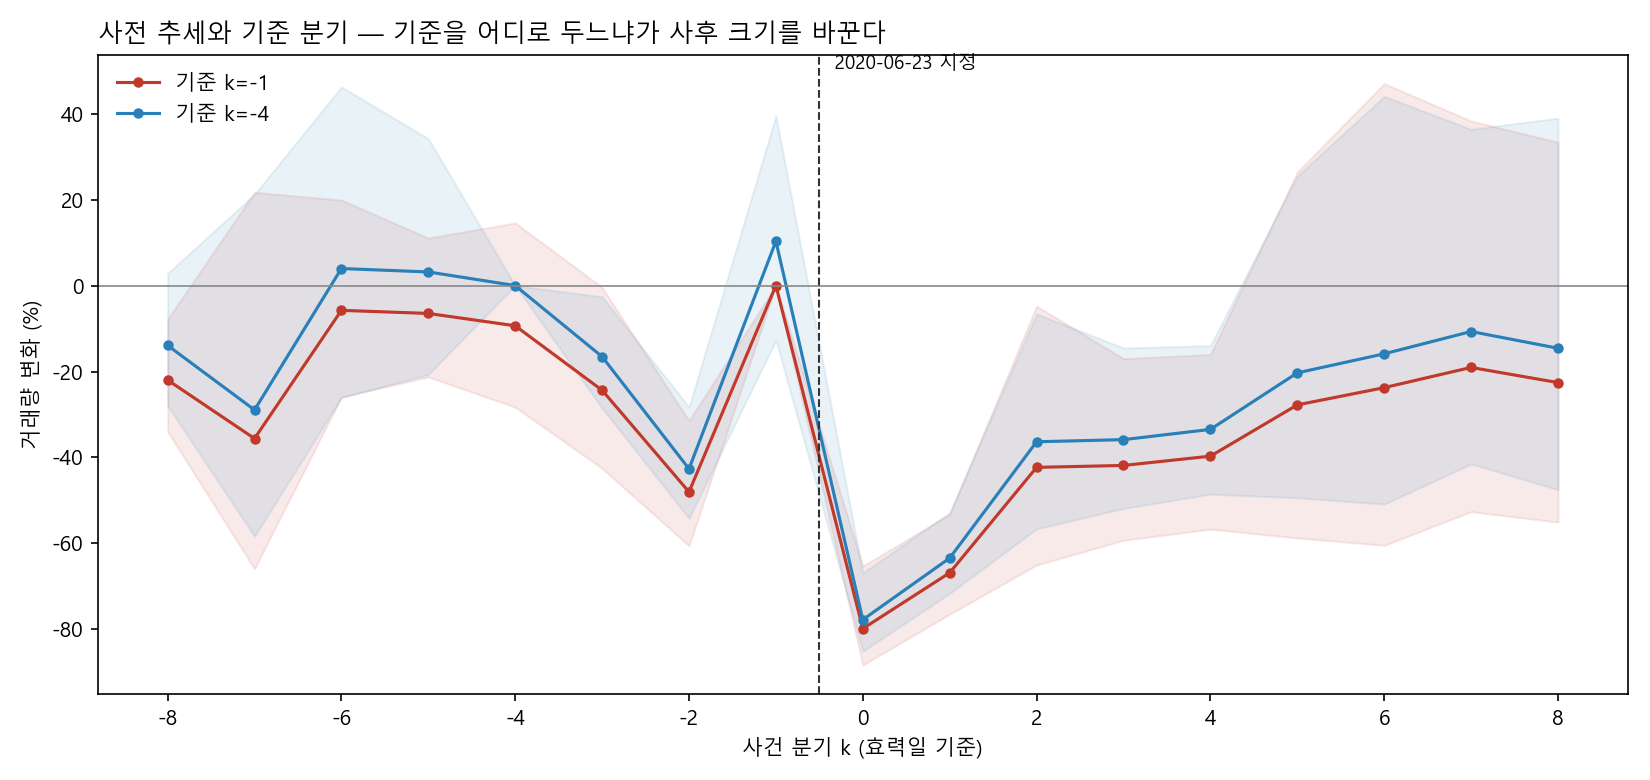
\includegraphics[width=\linewidth]{06d_pretrend.png}
  \caption{사전 추세 진단. 기준월 하나가 높았고 인접 두 분기가 반대로 흔들린다.}
  \label{fig:pretrend}
\end{figure}

\textbf{결정은 셋이다}(0014). 주 사양은 관행대로 $k=-1$을 유지한다. 지정 직후
효과는 \textbf{구간으로} 보고한다($-74 \sim -80\%$, 합성대조군까지 넣으면
$-71 \sim -80\%$). 그리고 \textbf{사후 $k \geq 4$는 해석하지 않는다} --- 기준
선택에 $-20 \sim +16\%$로 흔들리고 기울기 보정에도 부호가 뒤집힌다. ``효과가
얼마나 오래 갔는가''는 이 설계로 답할 수 없다.

\subsection{분석 구간}

인과추정 대상 기간을 \textbf{2025-10-19까지}로 한정한다(0002). 10·15 대책으로
2025-10-20부터 토허구역이 서울 25개 자치구 전체로 확대되어 \textbf{서울 안에
미처치 아파트가 존재하지 않는다.} 나흘 앞선 10-16에 규제지역도 서울 전역으로
확대되어 두 정책의 효과 분리도 불가능하다.

경기 미지정 지역을 통제군으로 쓰는 대안은 시장 구조가 달라 평행추세 방어가
어렵고, 경기 12개 지역도 동시에 지정되었다. \textbf{이 제약은 한계가 아니라 설계
근거다} --- 정책 타임라인을 읽고 식별 가능 구간을 스스로 잘라낸 판단이다.

\subsection{사전 등록한 예측}

6장에서 효과의 이질성이 허가 대상의 면적 기준에서 왔다는 결론에 이른다. 그
결론이 맞다면 \textbf{다른 자료에서 특정한 결과가 나와야 한다.} 그 예측을
결과를 보기 전에 적어 두었다(0022, 2026-09-18).

\begin{quote}
2025년 재지정은 허가 면적 기준이 6\,m$^2$이므로 소형 면제가 거의 없다.
면적 기준이 이질성의 원인이라면 \textbf{2025년에는 소형도 함께 줄어야 한다.}
\end{quote}

대출 가설이 맞았다면 2025년에도 소형은 줄지 않았어야 한다. 두 가설이 반대 방향을
예측하는 지점이다. 답은 6.8절에 있다.
